\documentclass{article}
\usepackage[margin=1in]{geometry}
\usepackage{amsmath,amsthm,amssymb}
\usepackage{bbm,enumerate,mathtools}
\usepackage{tikz,pgfplots}
\usepackage{chessboard}
\usepackage[hidelinks]{hyperref}
\usepackage{multicol} % Problem 35

\newenvironment{question}{\begin{trivlist}\item[\textbf{Question.}]}{\end{trivlist}}
\newenvironment{note}{\begin{trivlist}\item[\textbf{Note.}]}{\end{trivlist}}
\newenvironment{references}{\begin{trivlist}\item[\textbf{References.}]}{\end{trivlist}}
\newenvironment{related}{\begin{trivlist}\item[\textbf{Related.}]\end{trivlist}\begin{enumerate}}{\end{enumerate}}


\begin{document}
\rating{2}{2}
Consider the rectangles from Problem 29: those composed of $n$ squares such
that the greatest common divisor of all the sidelengths is 1. If rectangles
are measured by the longest side, the smallest rectangles are given by
$A295753$.
\begin{figure}[!h]
  \centering
  
\begin{tikzpicture}
    \draw[ultra thick, fill={rgb:white,3;red,0;green,2;blue,1}] (0,0) rectangle (1,1);
  \end{tikzpicture}\hspace{1cm}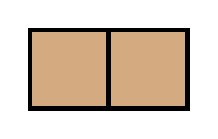
\begin{tikzpicture}
    \draw[ultra thick, fill={rgb:white,3;red,2;green,1;blue,0}] (0,0) rectangle (1,1);
    \draw[ultra thick, fill={rgb:white,3;red,2;green,1;blue,0}] (1,0) rectangle (2,1);
  \end{tikzpicture}
  \hspace{1cm}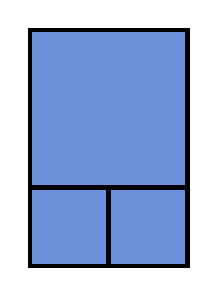
\begin{tikzpicture}
    \draw[ultra thick, fill={rgb:white,3;red,0;green,1;blue,3}] (0,0) rectangle (1,1);
    \draw[ultra thick, fill={rgb:white,3;red,0;green,1;blue,3}] (1,0) rectangle (2,1);
    \draw[ultra thick, fill={rgb:white,3;red,0;green,1;blue,3}] (0,1) rectangle (2,3);
  \end{tikzpicture}
  \hspace{1cm}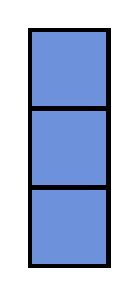
\begin{tikzpicture}
    \draw[ultra thick, fill={rgb:white,3;red,0;green,1;blue,3}] (0,0) rectangle (1,1);
    \draw[ultra thick, fill={rgb:white,3;red,0;green,1;blue,3}] (0,1) rectangle (1,2);
    \draw[ultra thick, fill={rgb:white,3;red,0;green,1;blue,3}] (0,2) rectangle (1,3);
  \end{tikzpicture}
  \hspace{1cm}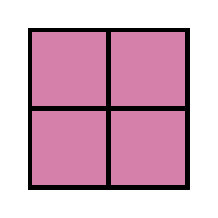
\begin{tikzpicture}
    \draw[ultra thick, fill={rgb:white,3;red,2;green,0;blue,1}] (0,0) rectangle (1,1);
    \draw[ultra thick, fill={rgb:white,3;red,2;green,0;blue,1}] (1,0) rectangle (2,1);
    \draw[ultra thick, fill={rgb:white,3;red,2;green,0;blue,1}] (0,1) rectangle (1,2);
    \draw[ultra thick, fill={rgb:white,3;red,2;green,0;blue,1}] (1,1) rectangle (2,2);
  \end{tikzpicture}
  \caption{
    Examples of $a(1) = 1$, $a(2) = 1$, $a(3) = 2$, and $a(4) = 1$.
  }
\end{figure}

\begin{question}
  How many distinct rectangles composed of $n$ squares have a longest side of
  $A295753(n)$?
\end{question}
\begin{related}
  \item Is the largest rectangle (as measured by smallest side) unique for large
  $n$?
  \item What if smallest rectangle is measured by perimeter?
\end{related}
\begin{note}
  Largest rectangles might be Fibonacci spirals, or they might be similar to the
  second example or the examples in the References.
\end{note}
\begin{references}
  \item \url{https://en.wikipedia.org/wiki/Squaring_the_square}
  \item \url{https://oeis.org/A295753}
\end{references}
\end{document}
